\chapter{散射理论}\label{ch:b3:scattering-theory}

我们对微观世界所知的几乎一切，
都是通过向它投射物体、观察反弹之物而获得的。卢瑟福
通过在硫化锌屏上计数α粒子闪光，发现了原子核；
五十年后，用更高能量的电子做同样的实验，
发现了质子内部的夸克。此后，核物理、粒子物理、
原子物理与凝聚态物理中的每一个\omterm{def:b3:scattering-theory:cross-section}{截面}，都要借助本章的理论来解读。
这里的语言是\emph{\omterm{def:b3:scattering-theory:cross-section}{截面}}——一个有效靶面积；
量子对象则是\emph{\omterm{thm:b3:scattering-theory:amplitude}{散射振幅}}，其\omterm{thm:b3:scattering-theory:born}{玻恩近似}给出一个令人难忘的结论：
弥散的靶在傅里叶空间中
逐角度地被探测。
在低能情形下，\omterm{thm:b3:scattering-theory:partial}{分波}起主导作用，
把任意复杂的势压缩为一个数——\omterm{thm:b3:scattering-theory:partial}{散射长度}——
如今它正被用来调控超冷量子气体；
而当投射粒子能够停留在准束缚态时，
\omterm{def:b3:scattering-theory:cross-section}{截面}会出现尖峰，即共振，
这是对原本不可见之物的谱学探测。

\section{截面}

\begin{definition}[截面]\label{def:b3:scattering-theory:cross-section}
\index{截面}\index{微分截面}
令通量为 $\Phi$（单位面积、单位时间内的粒子数）的均匀粒子束
射向一个靶粒子。散射入
立体角 $\dd\Omega$（中心方向为 $(\theta,
\varphi)$）的投射粒子速率定义了\emph{微分截面}，
\[
\dd\dot N = \Phi\,\frac{\dd\sigma}{\dd\Omega}\,\dd\Omega ,
\]
其积分 $\sigma = \int(\dd\sigma/\dd\Omega)\,\dd\Omega$ 即为
\emph{总截面}：靶有效呈现的
面积。对于单位体积内含 $n$ 个靶粒子的薄层，
束流按 $\eu^{-n\sigma x}$ 衰减：截面由
透出粒子的计数来确定。单位：核物理采用\emph{靶恩}，
$\qty{1}{b} = \qty{e-28}{m^2}$——大致相当于一个铀原子核的
几何尺寸，对中子而言“大如靶”。
\end{definition}

\begin{omfigure}
\begin{tikzpicture}[font=\small, >=Stealth]
  % incident plane wave
  \foreach \x in {-4.6,-4.0,-3.4,-2.8}
    \draw[omDef] (\x,-1.15) -- (\x,1.15);
  \draw[->, omDef, very thick] (-4.5,1.5) -- (-2.9,1.5);
  \node[omDef, anchor=south] at (-3.7,1.55) {光束，通量 $\Phi$};
  % target
  \fill[omThm] (0,0) circle (3pt);
  \node[anchor=north, font=\footnotesize] at (0,-0.18) {靶};
  % outgoing spherical
  \foreach \r in {0.7,1.3,1.9}
    \draw[omExo] (0,0) circle (\r);
  % detector
  \draw[->, thick] (0,0) -- (35:3.1);
  \draw[fill=omProp!25, draw=omProp, thick, rotate around={35:(35:3.4)}]
    ($(35:3.4)+(-0.12,-0.42)$) rectangle ($(35:3.4)+(0.12,0.42)$);
  \node[omProp, anchor=west, font=\footnotesize] at ($(35:3.4)+(0.25,0)$)
    {探测器，$\dd\Omega$};
  \draw (1.15,0) arc (0:35:1.15);
  \node at (17:1.5) {$\theta$};
  \draw[->, thick] (0,0) -- (2.6,0);
\end{tikzpicture}

{\small 散射实验：入射平面波、出射球面波，
位于角度 $\theta$ 处的探测器进行计数。计数的角分布
即反映了靶的物理性质。}
\end{omfigure}

\section{散射振幅与玻恩近似}

\begin{theorem}[散射态与振幅]\label{thm:b3:scattering-theory:amplitude}
\index{散射振幅}
对于能量为 $E = \hbar^2k^2/2m$ 的粒子，
与局域势 $V(\vect r)$ 相遇时，定态散射态在
远距离处渐近地表现为
\[
\psi(\vect r) \;\longrightarrow\;
\eu^{\iu kz} + f(\theta)\,\frac{\eu^{\iu kr}}{r} ,
\]
入射平面波加上出射球面波，后者由
\emph{\omterm{thm:b3:scattering-theory:amplitude}{散射振幅}} $f(\theta)$（量纲为长度）调制，并且
\[
\frac{\dd\sigma}{\dd\Omega} = |f(\theta)|^2 .
\]
\end{theorem}

\begin{proof}[部分证明]
$1/r$ 的衰减使得通过任一大球面的出射通量
为有限值；计算两项的\omterm{prop:b3:schrodinger-three-dimensions:current}{概率流}
（\cref{prop:b3:schrodinger-three-dimensions:current}），
单位立体角内的径向出射流为
$(\hbar k/m)|f|^2$，相对于入射通量 $\hbar k/m$，
二者之比即为 $\dd\sigma/\dd\Omega$ 的定义。此类
渐近形式的解之存在性在本阶段不加证明地承认。
\end{proof}

\begin{theorem}[玻恩近似]\label{thm:b3:scattering-theory:born}
\index{玻恩近似}\index{动量转移}
对于弱势（或快速投射粒子），
关于 $V$ 的一级\omterm{thm:b3:perturbation-theory:corrections}{微扰理论}给出
\[
f(\theta) = -\frac{m}{2\pi\hbar^2}
\int V(\vect r)\,\eu^{\iu\vect q\cdot\vect r}\,\dd^3r ,
\qquad
\vect q = \vect k - \vect k' , \quad
q = 2k\sin\frac\theta2 :
\]
在相差常数因子的意义下，振幅即为\emph{势的
傅里叶变换}在\omterm{thm:b3:scattering-theory:born}{动量转移} $\hbar\vect q$ 处的取值。
散射实验是物质的傅里叶分析器：
小角度读出长波长（粗结构），大角度读出
精细细节——这正是“能量更高”意味着
“距离更小”的最深层原因。
\end{theorem}

\begin{proof}[部分证明]
这是\omterm{thm:b3:perturbation-theory:golden}{费米黄金规则}
（\cref{thm:b3:perturbation-theory:golden}）在平面波
$\ket{\vect k} \to \ket{\vect k'}$ 之间的应用：矩阵元为
$\int V\eu^{\iu(\vect k - \vect k')\cdot\vect r}\dd^3r$，
末\omterm{prop:b3:schrodinger-three-dimensions:counting}{态密度}提供运动学因子，
其余的归并工作（承认）将它们组装成 $f$。弹性散射给出
$|\vect k'| = |\vect k|$，因而 $q = 2k\sin(\theta/2)$，
由 $\vect k, \vect k'$ 构成的等腰三角形可得。
\end{proof}

\begin{example}[从汤川势到卢瑟福散射]\label{ex:b3:scattering-theory:rutherford}
\index{卢瑟福散射}
对于屏蔽库仑势 $V = \dfrac{Q_1Q_2}{4\pi
\varepsilon_0 r}\,\eu^{-r/a}$，玻恩积分可以初等地算出
（见\cref{exo:b3:scattering-theory:5}），当屏蔽半径
$a \to \infty$ 时，
\[
\frac{\dd\sigma}{\dd\Omega} =
\Big(\frac{Q_1Q_2}{16\pi\varepsilon_0 E}\Big)^2
\frac{1}{\sin^4(\theta/2)} :
\]
即\emph{卢瑟福\omterm{def:b3:scattering-theory:cross-section}{截面}}。
由于 $1/r$ 势所特有的巧合，经典计算、\omterm{thm:b3:scattering-theory:born}{玻恩近似}与
精确量子结果三者完全一致——这正是卢瑟福
于 1911 年以经典方法算出正确公式，并
通过逐个闪烁的计数确认了原子核的存在
（见\cref{pb:b3:scattering-theory:1}）。
\end{example}

\section{分波与散射长度}

\begin{theorem}[相移]\label{thm:b3:scattering-theory:partial}
\index{分波}\index{相移}\index{散射长度}
对于中心势，将散射态按角动量分解：
每个\omterm{thm:b3:scattering-theory:partial}{分波} $l$ 离开势作用区时，
其径向振荡因相位 $\delta_l(k)$ 而\emph{发生平移}
——吸引使其提前，排斥使其延迟——并
可观测振幅重新组合为
\[
f(\theta) = \frac1k\sum_{l=0}^\infty(2l+1)\,\eu^{\iu\delta_l}
\sin\delta_l\,P_l(\cos\theta) , \qquad
\sigma = \frac{4\pi}{k^2}\sum_l(2l+1)\sin^2\delta_l .
\]
低能时，经典直觉（$l \sim kb$，
冲击参数 $b$）表明只有 $l = 0$ 的\omterm{thm:b3:scattering-theory:partial}{分波}能够穿透：散射
变得各向同性，且只由一个数决定，
\[
f \to -a , \qquad \sigma \to 4\pi a^2 ,
\]
其中 $a = -\lim_{k\to0}\delta_0/k$ 称为\emph{\omterm{thm:b3:scattering-theory:partial}{散射
长度}}。无论靶的内部结构多么复杂，低能时靶
\emph{就是}它的\omterm{thm:b3:scattering-theory:partial}{散射长度}——这一巨大的简化
正是冷原子物理所依赖的基础。
\end{theorem}
\admitted

\begin{omfigure}
\begin{tikzpicture}
  \begin{axis}[omaxis, axis x line=bottom, axis y line=left,
    width=11.6cm, height=5.2cm, xmin=0, xmax=12.3, ymin=-1.5, ymax=1.5,
    xlabel={$r$}, ylabel={$u_0(r)$},
    xlabel style={at={(axis description cs:0.5,-0.1)}, anchor=north},
    xtick=\empty, ytick=\empty, clip=false]
    \addplot[gray, dashed, domain=0:12.3, samples=200] {sin(deg(x))};
    \addplot[omDef, very thick, domain=1.9:12.3, samples=200] {sin(deg(x+0.9))};
    \draw[omExo, thick] (axis cs:0,-1.5) -- (axis cs:0,1.5);
    \fill[omExo!14] (axis cs:0,-1.5) rectangle (axis cs:1.9,1.5);
    \node[font=\scriptsize, anchor=south] at (axis cs:0.95,1.12) {势作用区};
    \node[font=\scriptsize, anchor=south] at (axis cs:0.95,0.78) {区域};
    \draw[<->, omThm, thick] (axis cs:8.51,-1.28) -- (axis cs:9.42,-1.28);
    \node[omThm, font=\scriptsize, anchor=north] at (axis cs:8.95,-1.32)
      {平移 $\delta_0/k$};
    \node[gray, font=\scriptsize, anchor=west] at (axis cs:10.7,1.28) {自由};
    \node[omDef, font=\scriptsize, anchor=west] at (axis cs:10.55,0.92) {散射后};
  \end{axis}
\end{tikzpicture}

{\small \omterm{thm:b3:scattering-theory:partial}{分波}离开相互作用区时，其振荡
已发生位移：\omterm{thm:b3:scattering-theory:partial}{相移} $\delta_0$。
探测器在某一能量下对中心势所能获知的
一切，就是这些\omterm{thm:b3:scattering-theory:partial}{相移}的集合。}
\end{omfigure}

\begin{example}[中子遇见质子]\label{ex:b3:scattering-theory:np}
慢中子与质子散射时，\omterm{def:b3:scattering-theory:cross-section}{截面} $\sigma \approx
\qty{20.4}{b}$——约为氘核几何尺寸所对应面积的
四十倍。解释如下：低能碰撞纯粹是 $s$ 波，
且包含两个自旋道，其实测\omterm{thm:b3:scattering-theory:partial}{散射长度}为
$a_{\text{t}} = \qty{5.4}{fm}$（三重态）与 $a_{\text{s}} =
\qty{-23.7}{fm}$（单态），二者都远大于
\qty{2}{fm} 的力程。$|a|$ 很大意味着存在一个\emph{几乎}
处于零能的态：三重态中几乎刚刚束缚的氘核
（见\cref{ex:b3:schrodinger-three-dimensions:deuteron}），以及单态中
一个恰好未能束缚的“虚”伙伴态——
其失败体现在 $a_{\text{s}} < 0$ 上。这一二十靶恩之谜，
由两个几乎束缚的态共同解决
（见\cref{exo:b3:scattering-theory:7}）。
\end{example}

\section{共振}

\begin{proposition}[布莱特–维格纳共振]\label{prop:b3:scattering-theory:resonance}
\index{共振!散射}\index{布莱特–维格纳公式}
若入射粒子能被暂时俘获到一个准束缚态中，
其能量为 $E_{\text{R}}$、寿命为 $\tau = \hbar/\Gamma$，
则相应的\omterm{thm:b3:scattering-theory:partial}{相移}扫过 $\pi/2$，并且
\omterm{thm:b3:scattering-theory:partial}{分波}\omterm{def:b3:scattering-theory:cross-section}{截面}出现尖峰：
\[
\sigma_l(E) \approx \frac{4\pi}{k^2}\,(2l+1)\,
\frac{\Gamma^2/4}{(E - E_{\text{R}})^2 + \Gamma^2/4} ,
\]
这是宽度为 $\Gamma$ 的洛伦兹峰，峰顶即波所能达到的
上限（“幺正性极限” $4\pi(2l+1)/k^2$）。倒过来看，
\omterm{def:b3:scattering-theory:cross-section}{截面}中的共振\emph{正是}某个态被发现的标志：
其位置即一个能级，其宽度即一个寿命。在
\cref{ch:b3:particle-physics}中，粒子动物园的大多数
成员正是以这样的峰被发现的。
\end{proposition}
\admitted

\begin{omfigure}
\begin{tikzpicture}
  \begin{axis}[omaxis, axis x line=bottom, axis y line=left,
    width=7.0cm, height=5.0cm, xmin=0, xmax=10, ymin=0, ymax=1.2,
    xlabel={$E$}, ylabel={$\sigma$（缩放后）},
    xlabel style={at={(axis description cs:0.5,-0.11)}, anchor=north},
    xtick={4}, xticklabels={$E_{\text{R}}$}, ytick=\empty, clip=false]
    \addplot[omDef, very thick, domain=0:10, samples=200]
      {0.06 + 0.25/((x-4)^2+0.27)};
    \draw[<->, omThm] (axis cs:3.48,0.53) -- (axis cs:4.52,0.53);
    \node[omThm, font=\scriptsize, anchor=south] at (axis cs:4.0,0.56) {$\Gamma$};
  \end{axis}
  \begin{axis}[omaxis, axis x line=bottom, axis y line=left,
    width=7.0cm, height=5.0cm, xmin=0, xmax=10, ymin=0, ymax=1.2,
    xshift=7.6cm,
    xlabel={$E$（eV）}, ylabel={$\sigma$（缩放后）},
    xlabel style={at={(axis description cs:0.5,-0.11)}, anchor=north},
    xtick={1}, ytick=\empty, clip=false]
    \addplot[omExo, very thick, domain=0.05:10, samples=250]
      {0.75*((x-1)*(x-1)+0.06)/(x*x*0.35+0.5)+0.02};
    \node[omExo, font=\scriptsize, anchor=west] at (axis cs:1.15,0.14)
      {透明窗口};
  \end{axis}
\end{tikzpicture}

{\small \omterm{thm:b3:scattering-theory:partial}{相移}的两个侧面。左：准束缚态
使 $\delta$ 穿过 $\pi/2$——一个布赖特–维格纳峰，其
宽度即一个寿命。右：拉姆绍尔–汤森效应——在
氩中，$\delta_0$ 穿过 $\pi$，发生在 \qty{1}{eV} 附近，使
原子对电子几乎透明：相消
干涉，即一种反共振。}
\end{omfigure}

\begin{method}[读懂散射问题]\label{met:b3:scattering-theory:method}
(1) 先看运动学：$k$，以及可达的 $q$ 范围 $0 \le q
\le 2k$——能看到哪些结构尺度？(2) 快而弱的情形：
用\omterm{thm:b3:scattering-theory:born}{玻恩近似}——对势作傅里叶变换，并检验其足够小。(3)
慢的情形：用\omterm{thm:b3:scattering-theory:partial}{分波}法，通常只取 $s$ 波；考虑\omterm{thm:b3:scattering-theory:partial}{散射长度}，
并期望 $\sigma = 4\pi a^2$（全同玻色子时：
$8\pi a^2$）。(4) $\sigma(E)$ 中的峰：拟合布赖特–维格纳公式，给出一个
能级和一个寿命；谷：相位穿过 $\pi$。(5) 扩展靶：
将点振幅乘以形状因子——即
密度的傅里叶变换
（见\cref{exo:b3:scattering-theory:12}）。
\end{method}

\begin{omfigure}
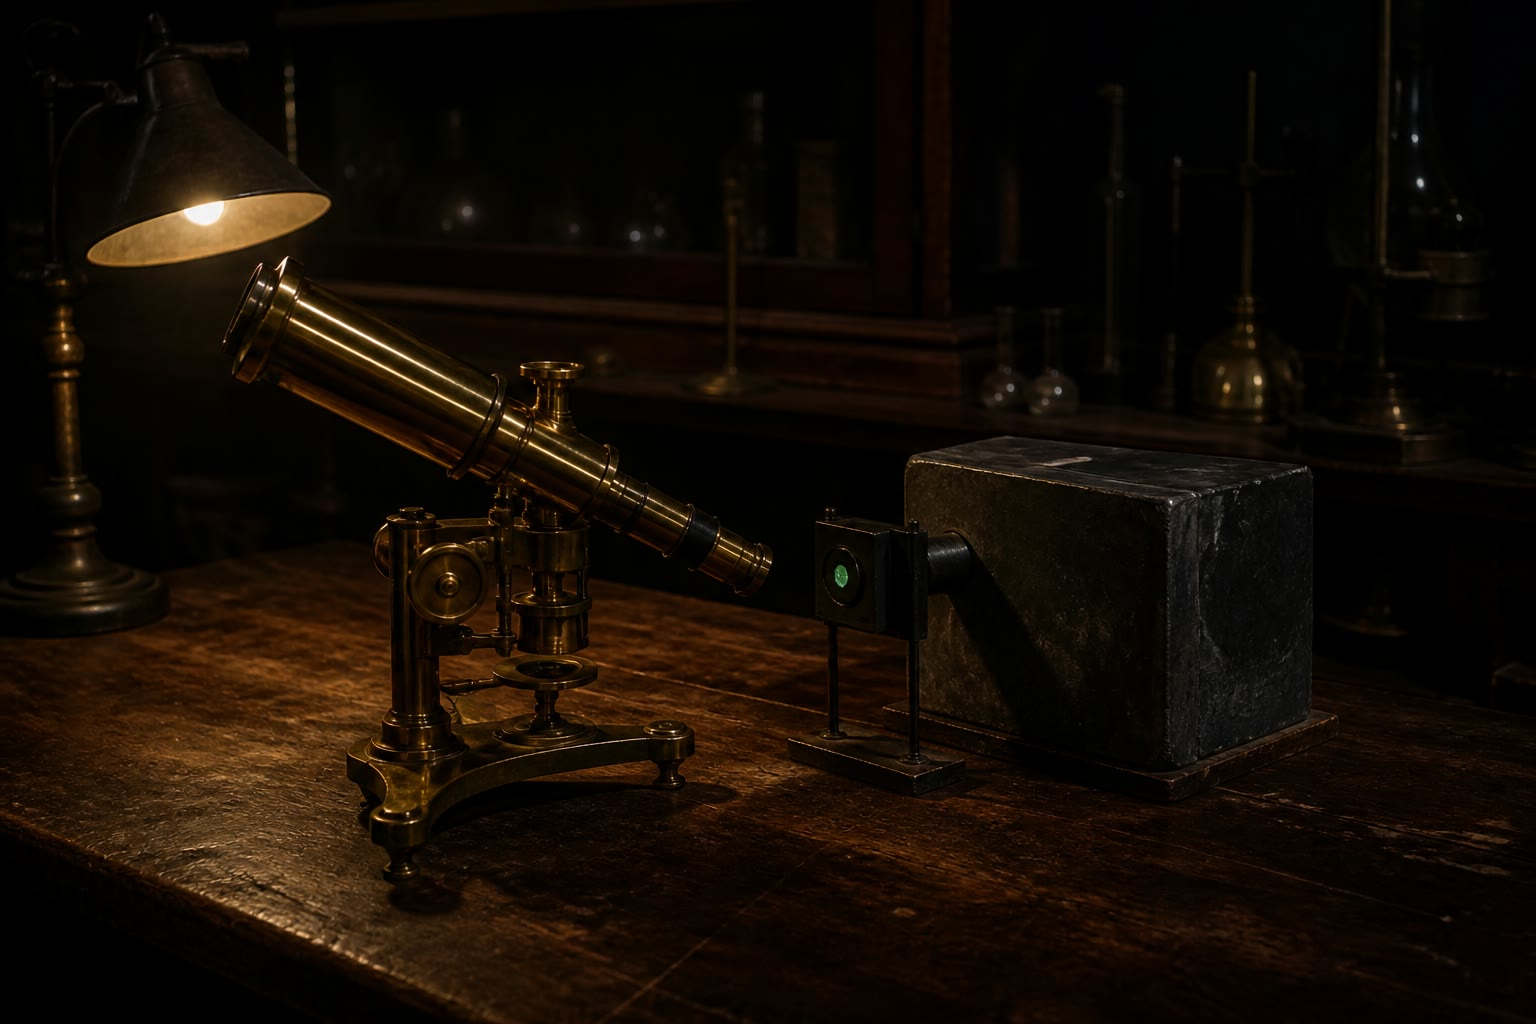
\includegraphics[width=0.58\linewidth]{images/book5/ai/b5-15-scintillation-lab.jpg}

{\small 第一台散射实验装置：一台黄铜显微镜对准硫化锌屏，每到达一个 $\alpha$ 粒子便计数一次微弱的绿色闪光。卢瑟福正是据此逐角计数，测定了原子核。}
\end{omfigure}

\section{练习}

\begin{exercise}[$\star$]\label{exo:b3:scattering-theory:1}
一束 \qty{1}{\micro A} 的质子束（$\num{6.2e12}$ 个质子/秒），
\omterm{def:b3:scattering-theory:cross-section}{截面}积为 \qty{1}{cm^2}，穿过一片 \qty{1}{\micro m} 厚的金箔（$n =
\qty{5.9e28}{m^{-3}}$）。(a) 靶的面密度。(b) 取
$\sigma = \qty{10}{b}$ 每个原子核，束流中
散射的比例为多少？(c) 若散射是各向同性的，进入立体角为
\qty{e-3}{sr} 的探测器的计数率。(d) 为什么
“\omterm{def:b3:scattering-theory:cross-section}{截面}”是\emph{这一组}
（投射粒子、靶、能量）的确定性质，而非仅属于靶本身？
\end{exercise}

\begin{exercise}[$\star$]\label{exo:b3:scattering-theory:2}
经典硬球，半径为 $R_1, R_2$：(a) 证明 $\sigma =
\pi(R_1 + R_2)^2$。(b) 对空气分子（$R \approx
\qty{0.15}{nm}$，$n = \qty{2.5e25}{m^{-3}}$），求平均自由程
$1/n\sigma$，算出其值，并与
本科一年级分册中的分子运动论结果比较。(c) 为何经典硬球不呈现
角度结构（$\dd\sigma/\dd\Omega$ 为常数——承认或
推导？）(d) 在\emph{量子}硬球散射中，哪一特征
（见\cref{exo:b3:scattering-theory:6}）没有
经典对应？
\end{exercise}

\begin{exercise}[$\star$]\label{exo:b3:scattering-theory:3}
\omterm{thm:b3:scattering-theory:born}{动量转移}。(a) 画出 $\vect k$、$\vect k'$ 构成的
三角形，并推导 $q = 2k\sin(\theta/2)$。(b) 对 \qty{5.5}{MeV} 的 α 粒子
（$k = \qty{1.0e15}{m^{-1}}$）：$q$ 在 $\theta \in
[0, \pi]$ 上的范围，以及可分辨的最小结构 $\sim 1/q_{\max}$。
(c) 对 \qty{500}{MeV} 的电子（$k \approx E/\hbar c$），同样求出。
(d) 归纳束流能量与显微镜分辨本领之间的联系。
\end{exercise}

\begin{exercise}[$\star$]\label{exo:b3:scattering-theory:4}
由\cref{thm:b3:scattering-theory:amplitude}出发：(a) 验证
$|f|^2$ 的量纲为面积与立体角之比；(b) 证明
穿过球面的散射通量为 $\Phi\sigma$；(c) 为什么
$f$ 一般必须为复数（其相位保证了哪一守恒律）？
(d) 写出光学定理 $\sigma_{\text{总}} =
(4\pi/k)\operatorname{Im}f(0)$，及其含义（前向波
必须恰好由散射出去的部分消耗掉）。
\end{exercise}

\begin{exercise}[$\star\star$]\label{exo:b3:scattering-theory:5}
汤川势的\omterm{thm:b3:scattering-theory:born}{玻恩近似}。取 $V(r) = \dfrac{g\,\eu^{-\mu r}}{r}$：(a)
计算玻恩积分（先算角度部分，再算 $\int_0^
\infty\sin(qr)\eu^{-\mu r}\dd r$），得到 $f = -\dfrac{2mg}
{\hbar^2(q^2 + \mu^2)}$。(b) 令 $\mu \to 0$，取 $g =
Q_1Q_2/4\pi\varepsilon_0$，并还原\omterm{ex:b3:scattering-theory:rutherford}{卢瑟福散射}。(c) 为什么
\emph{总}卢瑟福\omterm{def:b3:scattering-theory:cross-section}{截面}会发散，哪一物理因素
（原子电子的屏蔽）使结果恢复为有限值？
(d) 在粒子物理中，以 $\mu =
m_\pi c/\hbar$ 的汤川形式模拟核力：计算其作用范围
$1/\mu$，取 $m_\pi c^2 = \qty{140}{MeV}$。
\end{exercise}

\begin{exercise}[$\star\star$]\label{exo:b3:scattering-theory:6}
量子硬球（半径 $a$），$s$ 波：外部 $u_0 =
\sin(kr + \delta_0)$，且 $u_0(a) = 0$。(a) 证明 $\delta_0 = -ka$。
(b) 证明 $\sigma \to 4\pi a^2$（$k \to 0$），即
几何阴影的\emph{四}倍。(c) 给出该因子的波动解释
（长波长时衍射没有清晰阴影）。(d) 高能时，
答案趋于 $2\pi a^2$，仍为几何阴影的两倍
（阴影衍射）：为何绝不只是 $\pi a^2$？
\end{exercise}

\begin{exercise}[$\star\star$]\label{exo:b3:scattering-theory:7}
氢的二十靶恩。慢速非极化中子与
质子碰撞时，三重态道的权重为 $3/4$，而
单态道的权重为 $1/4$：$\sigma = \pi(3a_{\text{t}}^2 +
a_{\text{s}}^2)$。（a）取 $a_{\text{t}} = \qty{5.4}{fm}$，
$a_{\text{s}} = \qty{-23.7}{fm}$，计算其值，并与
实测 \qty{20.4}{b} 比较。（b）哪一道占主导，
尽管其统计权重较小？（c）联系 $a_{\text{t}}$ 的大小与符号，
与氘核近零结合能的关系；$a_{\text{s}} < 0$ 说明
单态体系具有怎样的性质？（d）为何水是反应堆中子的有效
慢化剂——为何该\omterm{def:b3:scattering-theory:cross-section}{截面}
对它至关重要？
\end{exercise}

\begin{exercise}[$\star\star$]\label{exo:b3:scattering-theory:8}
拉姆绍尔–汤森效应。将氩原子对入射电子建模为
一个吸引性方势阱，作用范围 $R =
\qty{0.2}{nm}$。（a）阱内波数为 $K =
\sqrt{2m(E + V_0)}/\hbar$；匹配可使外部波
恰好以 $\delta_0 = \pi$ 出射——此时 $s$ 波
\omterm{def:b3:scattering-theory:cross-section}{截面}为多少？（b）为何原子在该能量下几乎不可见，
尽管势阱很深？（c）估计 $V_0$，使透明点
接近 $E = \qty{1}{eV}$（使势阱恰容纳半个波长：
$KR \approx \pi$）。（d）为何氦和
氖在可比能量下\emph{不}显示该效应（它们的
势阱过浅，无法使 $\delta_0$ 达到 $\pi$）——这种效应的存在
本身证明了关于物质波的什么？
\end{exercise}

\begin{exercise}[$\star\star$]\label{exo:b3:scattering-theory:9}
对纯 $s$ 波，\omterm{thm:b3:scattering-theory:amplitude}{散射振幅} $f = \eu^{\iu\delta_0}\sin\delta_0/
k$：（a）计算 $\sigma$；（b）计算 $(4\pi/k)\operatorname{Im}
f(0)$，验证光学定理；（c）证明最大
$s$ 波\omterm{def:b3:scattering-theory:cross-section}{截面}为 $4\pi/k^2$（幺正性极限），并
对热中子（$k = \qty{3.1e10}{m^{-1}}$）计算该值，以靶恩计；
（d）为何共振无论相互作用多强，都无法使 $\sigma_0$ 越过
该上限？
\end{exercise}

\begin{exercise}[$\star\star\star$]\label{exo:b3:scattering-theory:10}
中子共振。铀-238 对中子有一个著名的共振，
位于 $E_{\text{R}} = \qty{6.67}{eV}$ 处，总宽度
为 $\Gamma = \qty{27}{meV}$。（a）计算该共振的寿命。
（b）计算该能量下的 $4\pi/k^2$，以靶恩计，
并与实测峰值 $\sim\qty{2e4}{b}$ 比较（其差异即
弹性道与俘获道之间的分支因子——
请加以说明）。（c）以温度为单位表示的宽度：为何多普勒
展宽随燃料温度的变化对反应堆稳定性至关重要
（何种符号的反馈）？（d）用两句话说明：
此类共振如何使 $^{238}$U 在超热区成为中子
吸收体，以及为何这对反应堆设计至关重要。
\end{exercise}

\begin{exercise}[$\star\star\star$]\label{exo:b3:scattering-theory:11}
冷原子只取决于一个数。（a）对全同玻色子，
低能\omterm{def:b3:scattering-theory:cross-section}{截面}为 $8\pi a^2$（相长交换
干涉——直接采用此结果）：对铷取 $a =
100\,a_0$ 计算。（b）在 $T = \qty{100}{nK}$ 下，检验 $ka \ll 1$
（计算 $k$，依据 $k_{\text{B}}T = \hbar^2k^2/2m$，$m =
\qty{1.4e-25}{kg}$）：气体真正只依赖于 $a$。
（c）在“费什巴赫”共振附近，磁场将一个
分子能级拖过零能，$a$ 发散并变号，
正如\cref{ex:b3:scattering-theory:np}所示：气体的相互作用
能否随意改变？（d）为何这种可调性——相互作用强度如旋钮般可调——是
物理学家梦寐以求的
仪器（举一用途：制备分子、模拟强耦合物质、
使凝聚体坍缩）？
\end{exercise}

\begin{exercise}[$\star\star\star$]\label{exo:b3:scattering-theory:12}
形状因子：称量电荷云。对延展的电荷
密度 $\rho(\vect r)$，玻恩振幅对点状结果
乘以 $F(q) = \int\rho(\vect r)\eu^{\iu\vect q\cdot\vect r}
\dd^3r/Q$。（a）证明 $F(0) = 1$。（b）对小 $q$ 展开：$F
\approx 1 - q^2\langle r^2\rangle/6$：测量低 $q$ 处的
下降，即可称出 $\langle r^2\rangle$。（c）电子–质子
散射拟合得 $\sqrt{\langle r^2\rangle} \approx \qty{0.84}{fm}$：
哪一项独立测量可以印证它（μ子氢，
见\cref{pb:b3:hydrogen-atom:1}），
以及它们历史上的分歧（“质子半径
之谜”）为何如此受重视？（d）当 $q \gg 1/r_{\text{p}}$ 时，
弹性形状因子随之衰减，但硬散射仍
来自\emph{点状组分}：用一句话说明 1968 年
卢瑟福实验的深度非弹性版本在
质子内部发现了什么。
\end{exercise}

\section{问题：发现原子核的闪光计数员}

\begin{problem}[{周末问题——卢瑟福散射，从
几何到夸克}]\label{pb:b3:scattering-theory:1}
1909 年，盖革与马斯登坐在暗室中计数闪烁
的闪光：α 粒子射向金箔，少数
几乎原路弹回——“仿佛一发炮弹被薄纸
弹了回来”。卢瑟福 1911 年对这些计数的分析
建立了核式原子模型。本题重建这一过程。数据：α 粒子能量 $E =
\qty{5.5}{MeV}$，电荷 $z = 2$；金的 $Z = 79$，箔厚 $t
= \qty{0.4}{\micro m}$, $n = \qty{5.9e28}{\text{原子}/m^3}$; $k_C =
1/4\pi\varepsilon_0 = \qty{8.99e9}{N.m^2/C^2}$.

\medskip\noindent\textbf{第一部分——一个 α 粒子，一个原子核。}
\begin{enumerate}
  \item 在葡萄干布丁模型中（电荷分布于整个原子，
        \qty{e-10}{m}），估算单个原子能
        给予一个 \qty{5.5}{MeV} 的 α 粒子的最大偏转（涂抹均匀的球体
        的场：$\theta \sim$ 力 $\times$ 时间 / 动量
        $\sim 2Zze^2k_C/(E\cdot\qty{e-10}{m})$，单位为弧度）。这类
        碰撞的任意累积能否使 α 粒子向后散射？
  \item 现设电荷集中于一点。写出正碰撞时的
        最近距离 $d_0$（动能全部转化为
        库仑能），并计算其值。
  \item 若近反向散射的速率可测得，
        因此\emph{立即}说明原子正电荷的
        集中程度如何？
  \item 对一般的碰撞参数 $b$，经典轨道
        给出 $\tan(\theta/2) = d_0/2b$（在本阶段不加证明地承认——即
        本科一年级分册引力一章中的双曲线，取斥力情形）：检验其在
        $b \to 0$ 与 $b \to
        \infty$ 时的极限。
  \item 求使 α 粒子偏转
        超过 $90^\circ$ 的碰撞参数，以及穿过金箔的 α 粒子中
        与某一原子核的距离小于该参数的比例（$n t\,\pi
        b^2$）。
  \item 盖革与马斯登发现，约每 8000 个 α 粒子中有 1 个
        偏转超过 $90^\circ$：请与上述结果比较。
\end{enumerate}

\medskip\noindent\textbf{第二部分——\omterm{def:b3:scattering-theory:cross-section}{截面}。}
\begin{enumerate}[resume]
  \item 瞄准距离位于 $[b, b + \dd b]$ 内的 α 粒子散射
        到 $[\theta, \theta + \dd\theta]$ 内：由 $\dd\sigma =
        2\pi b\,|\dd b|$ 及轨道关系式，导出
        \[
        \frac{\dd\sigma}{\dd\Omega} =
        \Big(\frac{d_0}{4}\Big)^2\frac{1}{\sin^4(\theta/2)} .
        \]
  \item 验证该结果与
        \cref{ex:b3:scattering-theory:rutherford}中的玻恩/量子结果一致（将 $d_0$
        用 $E$ 表示）。
  \item 计算 $\dd\sigma/\dd\Omega$ 在 $\theta = 30^\circ$、
        $60^\circ$、$120^\circ$ 处的值（单位为靶恩每球面度）。
  \item 盖革与马斯登 1913 年在几何条件固定时的计数
        正比于 $1{:}\,\sin^{-4}(\theta/2)$：计算
        $30^\circ$ 与 $120^\circ$ 之间的预测计数比，并
        指出
        他们的数据在五个数量级的
        计数率范围内都遵循这样的比值。
  \item 同一公式中的 $Z^2$ 为何使实验能够
        \emph{称量}原子核的电荷——这类拟合如何帮助
        将金（79 号元素）的 $Z$ 确定为原子序数？
  \item $1/E^2$ 的含义是什么：当 α 粒子的能量加倍时，
        整个角分布将发生怎样的变化？
\end{enumerate}

\medskip\noindent\textbf{第三部分——原子核的大小。}
\begin{enumerate}[resume]
  \item 角度 $\theta$ 处的最近接近距离：$d(\theta) =
        \tfrac{d_0}2[1 + 1/\sin(\theta/2)]$（承认此结果）。计算
        $\theta = 180^\circ$ 及 \qty{60}{\degree} 时的值。
  \item 只要 $d(\theta)$ 大于原子核半径，点电荷公式便成立：
        金原子核的大小有怎样的上界？
        卢瑟福验证过的 $180^\circ$ 数据
        确立了这一上界。
  \item 使用能量更高的入射粒子时，大角度处的计数
        \emph{低于}卢瑟福的预言：这种偏离说明存在
        什么新的力，作用距离为多少？
  \item 现代电子散射给出原子核半径 $R
        \approx r_0A^{1/3}$，其中 $r_0 = \qty{1.2}{fm}$：计算金（$A = 197$）的值，
        并与你得到的上界比较。
  \item $A^{1/3}$ 说明了核物质的密度具有怎样的性质
        （恒定？还是增长？）——这一事实是
        \cref{ch:b3:nuclear-physics}将要建立其上的基础。
  \item 为何（不辨电荷的）葡萄干布丁模型是因
        \emph{这一}实验而被推翻，而非因光谱学？
\end{enumerate}

\medskip\noindent\textbf{第四部分——卢瑟福的后代。}
\begin{enumerate}[resume]
  \item 列出 1911 年与 1968 年之间精确的对照表：
        α 粒子 $\to$ 电子束，金原子 $\to$ 质子，
        原子核 $\to$ 夸克——在 SLAC 中，谁扮演了
        “意料之外的大角度事件”的角色？
  \item 为何\emph{电子}是更干净的探针（α 粒子与原子核散射
        中存在哪种复杂情况，而电子不具有
        这种情况？）
  \item 用玻恩的语言来说：高 $q$ 下的弹性散射测得形状因子的坍缩
        （一团柔软的云），而深度非弹性散射的速率
        仍然很大且近似点状：
        请陈述由此得出的结论。
  \item 用三行概括百年的历程：给出
        （探针能量，可分辨距离），分别对应 1911 年 α 粒子（$\sim\qty{e-14}{m}$）、
        1968 年 SLAC（\qty{20}{GeV}，$\sim\qty{e-16}{m}$）以及
        LHC（TeV 能标，$\sim\qty{e-19}{m}$）的情形，
        使用规则“分辨率 $\sim \hbar c/(qc)$”。
  \item 中子不带电，只与原子核（以及磁矩）发生散射：说出中子散射
        因而能在 X 射线难以看清的材料中揭示的两种东西
        （如氢等轻原子；
        磁有序）。
  \item LHC 的发现\omterm{def:b3:scattering-theory:cross-section}{截面}以
        \emph{飞靶恩}（$\qty{e-43}{m^2}$）为单位测量：从靶恩到
        飞靶恩相差十五个数量级——这说明
        有趣的碰撞有多罕见，
        以及为何亮度（输送的通量）与能量
        同样珍贵？
  \item 总结这一命名结果：$\sin^{-4}(\theta/2)$ 定律
        经逐次闪烁验证，使原子 $99.98\%$ 的质量
        被压入其尺度的 $10^{-14}$ 体积之内——而同一实验
        在不断加强的条件下重复进行，始终在
        发现下一层结构。
\end{enumerate}
\end{problem}
